% This LaTeX was auto-generated from MATLAB code.
% To make changes, update the MATLAB code and export to LaTeX again.

\documentclass{article}

\usepackage[utf8]{inputenc}
\usepackage[T1]{fontenc}
\usepackage{lmodern}
\usepackage{graphicx}
\usepackage{color}
\usepackage{hyperref}
\usepackage{amsmath}
\usepackage{amsfonts}
\usepackage{epstopdf}
\usepackage[table]{xcolor}
\usepackage{matlab}
\usepackage[paperheight=795pt,paperwidth=614pt,top=72pt,bottom=72pt,right=72pt,left=72pt,heightrounded]{geometry}

\sloppy
\epstopdfsetup{outdir=./}
\graphicspath{ {./lab_2_media/} }

\begin{document}

\matlabtitle{Задание 1}

\begin{matlabcode}
y_0_arr = [ 1 1 1 0.05 0.05 0 ];
dot_y_0_arr = [ 0 0 0 0 0 0.1 ];
lambda_1_arr = [ -4.5 -3.7+5i 29i 0.7+5i 4.5 -2.8 ];
lambda_2_arr = [ -5.5 -3.7-5i -29i 0.7-5i 5.5 2.8 ];
\end{matlabcode}

\begin{par}
\begin{flushleft}
Выведем общую формулу для вычисления $a_0 ,a_1$:
\end{flushleft}
\end{par}

\begin{par}
\begin{flushleft}
Характеристическое уравнение: $\lambda^2 +a_1 \lambda +a_0 =0$
\end{flushleft}
\end{par}

\begin{par}
\begin{flushleft}
Получим систему:
\end{flushleft}
\end{par}

\begin{par}
$$\left\lbrace \begin{array}{c}
a_1 =-\lambda_1 -\lambda_2 \\
a_0 =\lambda_1 \cdot \lambda_2 
\end{array}\right.$$
\end{par}

\begin{par}
\begin{flushleft}
Вычислим коэффициеты:
\end{flushleft}
\end{par}

\begin{matlabcode}
a_0_arr = zeros(1, 6);
a_1_arr = zeros(1, 6);

for k = 1:6
    a_1_arr(k) = - lambda_1_arr(k) - lambda_2_arr(k);
    a_0_arr(k) = lambda_1_arr(k) * lambda_2_arr(k);
end
fprintf('№  a_1\t\t a_0\n');
\end{matlabcode}
\begin{matlaboutput}
№  a_1		 a_0
\end{matlaboutput}
\begin{matlabcode}
for k = 1:6
    fprintf('%1i %7.3f\t%7.3f\n', ...
        k, real(a_1_arr(k)), real(a_0_arr(k)));
end
\end{matlabcode}
\begin{matlaboutput}
1  10.000	 24.750
2   7.400	 38.690
3   0.000	841.000
4  -1.400	 25.490
5 -10.000	 24.750
6   0.000	 -7.840
\end{matlaboutput}

\begin{par}
\begin{flushleft}
Получаем:
\end{flushleft}
\end{par}

\begin{par}
\begin{flushleft}
\texttt{№  a\_1		 a\_0}
\end{flushleft}
\end{par}

\begin{par}
\begin{flushleft}
\texttt{1  10.000	 24.750}
\end{flushleft}
\end{par}

\begin{par}
\begin{flushleft}
\texttt{2   7.400	 38.690}
\end{flushleft}
\end{par}

\begin{par}
\begin{flushleft}
\texttt{3   0.000	841.000}
\end{flushleft}
\end{par}

\begin{par}
\begin{flushleft}
\texttt{4  -1.400	 25.490}
\end{flushleft}
\end{par}

\begin{par}
\begin{flushleft}
\texttt{5 -10.000	 24.750}
\end{flushleft}
\end{par}

\begin{par}
\begin{flushleft}
\texttt{6   0.000	 -7.840}
\end{flushleft}
\end{par}

\begin{par}
\begin{flushleft}
\texttt{Перепишем наше ДУ в более удобном виде для построения схемы:}
\end{flushleft}
\end{par}

\begin{par}
$$p^2 y+a_1 py+a_0 y=a_0 u\Rightarrow y=-\frac{1}{p}(a_1 y+\frac{1}{p}a_0 (y-u))$$
\end{par}

\begin{par}
\begin{flushleft}
Найдём аналитическое выражение для свободной составляющей движения системы $y_{\textrm{св}} (t)$ для каждого варианта:
\end{flushleft}
\end{par}

\begin{par}
\begin{flushleft}
1. $\begin{array}{l}
\left\lbrace \begin{array}{c}
y_{св} (t)=C_1 e^{-4.5t} +C_2 e^{-5.5t} \\
y(0)=1\\
\dot{y} (0)=0
\end{array}\right.\Rightarrow \left\lbrace \begin{array}{c}
C_1 +C_2 =1\\
-4.5C_1 -5.5C_2 =0
\end{array}\right.\Rightarrow \left\lbrace \begin{array}{c}
C_1 =5.5\\
C_2 =-4.5
\end{array}\right.\\
y_{св} (t)=5.5e^{-4.5t} -4.5e^{-5.5t} 
\end{array}$
\end{flushleft}
\end{par}


\vspace{1em}
\begin{par}
\begin{flushleft}
2. $\left\lbrace \begin{array}{c}
y_{св} (t)=e^{-3.7t} (C_1 \sin (5t)+C_2 \cos (5))\\
y(0)=1\\
\dot{y} (0)=0
\end{array}\right.\Rightarrow \left\lbrace \begin{array}{c}
\end{array}\right.$
\end{flushleft}
\end{par}


\vspace{1em}
\begin{par}
\begin{flushleft}
3. $\left\lbrace \begin{array}{c}
y_{св} (t)=C_1 \sin (29t)+C_2 \cos (29t)\\
y(0)=1\\
\dot{y} (0)=0
\end{array}\right.\Rightarrow \left\lbrace \begin{array}{c}
\end{array}\right.$
\end{flushleft}
\end{par}


\vspace{1em}
\begin{par}
\begin{flushleft}
4. $\left\lbrace \begin{array}{c}
y_{св} (t)=e^{-0.7t} (C_1 \sin (5t)+C_2 \cos (5))\\
y(0)=0.05\\
\dot{y} (0)=0
\end{array}\right.\Rightarrow \left\lbrace \begin{array}{c}
\end{array}\right.$
\end{flushleft}
\end{par}


\vspace{1em}
\begin{par}
\begin{flushleft}
5. $\left\lbrace \begin{array}{c}
y_{св} (t)=C_1 e^{5.5t} +C_2 e^{4.5t} \\
y(0)=0.05\\
\dot{y} (0)=0
\end{array}\right.\Rightarrow \left\lbrace \begin{array}{c}
\end{array}\right.$
\end{flushleft}
\end{par}


\vspace{1em}
\begin{par}
\begin{flushleft}
6. $\left\lbrace \begin{array}{c}
y_{св} (t)=C_1 e^{2.8t} +C_2 e^{-2.8t} \\
y(0)=0\\
\dot{y} (0)=0.1
\end{array}\right.\Rightarrow \left\lbrace \begin{array}{c}
\end{array}\right.$
\end{flushleft}
\end{par}

\begin{matlabcode}
y_fm_array = {@y_fm_1};
simtime = 10;
time_interval = linspace(0, simtime, 10000);

y = y_fm_array{1}(time_interval);
dot_y_0 = dot_y_0_arr(1);
y_0 = y_0_arr(1);
a_0 = a_0_arr(1);
a_1 = a_1_arr(1);
plot_1 = sim("lab_2_1.slx", simtime);
plot(plot_1.y.Time, plot_1.y.Data, LineWidth=2, LineStyle="-");
hold on;
plot(time_interval, y, LineWidth=2, LineStyle="--");

%xlim([-0.1 10.00]);
%ylim([0.00 1.25]);
grid on;
legend("$fuck$", Location="best", FontSize=14, Interpreter="latex");
xlabel("$t, c$", Interpreter="latex");
ylabel("$Signal$", Interpreter="latex");
set(gcf, Position=[100, 100, 1200, 600]);
set(gca, FontSize=14); 
hold off;
exportgraphics(gcf, 'images/plot_1.png', Resolution=200);
\end{matlabcode}
\begin{center}
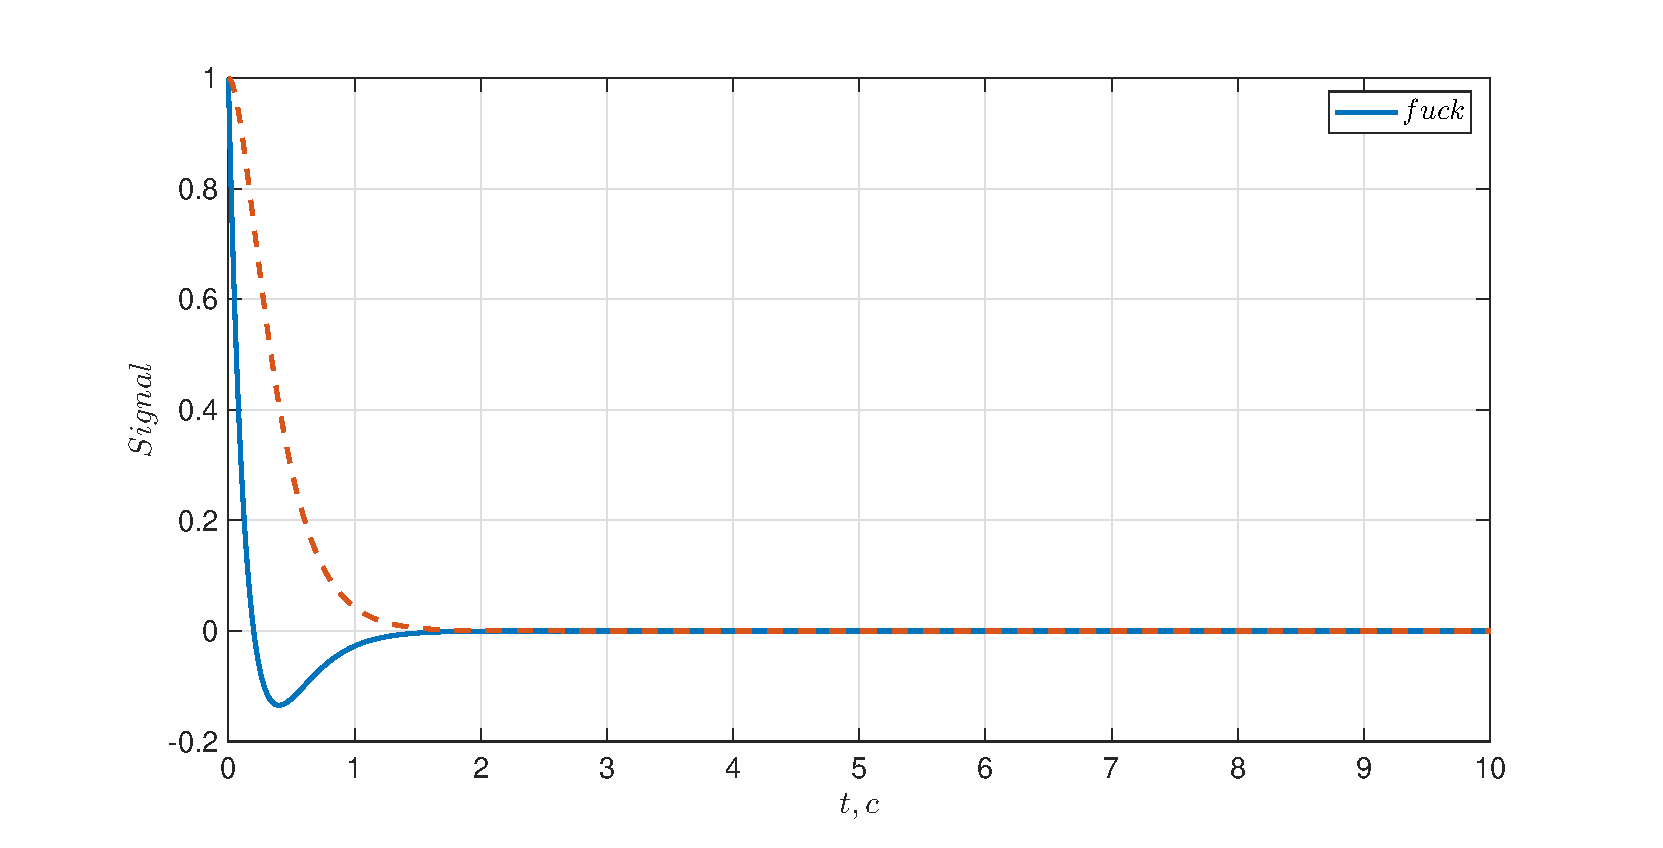
\includegraphics[width=\maxwidth{120.42147516307075em}]{figure_0.eps}
\end{center}


\begin{matlabcode}
function y = y_fm_1(t)
    y = 5.5 .* exp(-4.5 .* t) - 4.5 .* exp(-5.5 .* t);
end
\end{matlabcode}

\end{document}
